\section{Auswertung}
\label{sec:Auswertung}

\subsection{Untergrundstrom und die Strom-Temperatur-Kurve}
Die aufgenommenen Messwerte für die KBr($\SI{0.05}{\percent \mole}$ SR) -Probe sind in \autoref{tab:daten_15} für die Heizrate $b = \SI{1.5}{\kelvin \per \minute}$ und in \autoref{tab:daten_20} für $b = \SI{2.0}{\kelvin \per \minute}$ gelistet.
Im folgenden wird das Vorzeichen des Heizstrom umdefiniert und der Offset des Picoampere-Meters $I_{off, 1.5} = \SI{5}{\pico\ampere}$ für $b = \SI{1.5}{\kelvin \per \minute}$ bzw. $I_{off, 2.0} = \SI{3.5}{\pico\ampere}$ für $b = \SI{2.0}{\kelvin \per \minute}$ addiert:
\begin{equation*}
    I = I_\text{raw} \cdot (-1) + I_{off, b}
\end{equation*}
\begin{table}
    \centering
    \begin{tabular}{S[table-format=2.0] S[table-format=2.0] S[table-format=2.0] |}
        \toprule
        $t \,/\, \si{minute}$ & $T \,/\, \si{\degreeCelsius}$ & $I \,/\, \si{\pico\ampere}$ \\
        \midrule
        0 & -48.8 & 4.2 \\
        1 & -46.8 & 4.2 \\
        2 & -44.8 & 4.2 \\
        3 & -43 & 4.1 \\
        4 & -41 & 4.0 \\
        5 & -39.6 & 3.9 \\
        6 & -38 & 3.7 \\
        7 & -36.5 & 3.5 \\
        8 & -35.1 & 3.3 \\
        9 & -33.9 & 3.1 \\
        10 & -32.5 & 2.7 \\
        11 & -31.3 & 2.3 \\
        12 & -29.9 & 1.8 \\
        13 & -28.4 & 1.2 \\
        14 & -26.7 & 0.4 \\
        15 & -25.1 & -0.7 \\
        16 & -23.5 & -1.9 \\
        17 & -22 & -3.2 \\
        18 & -20.5 & -4.5 \\
        19 & -19.1 & -5.7 \\
        20 & -17.7 & -6.7 \\
        21 & -16.3 & -7.6 \\
        22 & -14.8 & -8.3 \\
        23 & -13.3 & -8.6 \\
        24 & -11.5 & -8.5 \\
        25 & -10 & -7.8 \\
        26 & -8.4 & -6.6 \\
        27 & -6.9 & -5.2 \\
        28 & -5.4 & -3.8 \\
        29 & -3.9 & -2.6 \\
        30 & -2.5 & -1.8 \\
        31 & -1.3 & -1.3 \\
        32 & -0.1 & -1 \\
        33 & 1.3 & -1.1 \\
        \bottomrule
    \end{tabular}
    \begin{tabular}{| S[table-format=2.0] S[table-format=2.0] S[table-format=2.0]}
        \toprule
        $t \,/\, \si{minute}$ & $T \,/\, \si{\degreeCelsius}$ & $I \,/\, \si{\pico\ampere}$ \\
        \midrule
        34 & 2.9 & -1.3 \\
        35 & 4.5 & -1.7 \\
        36 & 6.3 & -2.2 \\
        37 & 7.8 & -2.7 \\
        38 & 9.3 & -3.2 \\
        39 & 10.8 & -3.5 \\
        40 & 12.2 & -3.9 \\
        41 & 13.5 & -4.3 \\
        42 & 15 & -4.9 \\
        43 & 16.5 & -5.5 \\
        44 & 18 & -6.2 \\
        45 & 19.4 & -7.6 \\
        46 & 21 & -7.9 \\
        47 & 22.5 & -9 \\
        48 & 24 & -11 \\
        49 & 25.5 & -11.5 \\
        50 & 27 & -13.5 \\
        51 & 28.5 & -15 \\
        52 & 30 & -17 \\
        53 & 31.5 & -19 \\
        54 & 33 & -21.5 \\
        55 & 34.5 & -24 \\
        56 & 36.1 & -27 \\
        57 & 37.7 & -29 \\
        58 & 39.2 & -31 \\
        59 & 40.6 & -32.5 \\
        60 & 42 & -33 \\
        61 & 43.3 & -32 \\
        62 & 44.8 & -31.5 \\
        63 & 46.5 & -30.5 \\
        64 & 48.2 & -28.5 \\
        65 & 49.6 & -26.5 \\
        66 & 51.1 & -22.5 \\
        & & \\
        \bottomrule
    \end{tabular}
    \caption{Temperatur $T$ und Heizstrom $I$ in Abhängigkeit der Zeit $t$ bei einer Heizrate von $b = \SI{1.5}{\frac{\degreeCelsius}{\minute}}$.}
    \label{tab:daten_15}
\end{table}

\begin{table}
    \centering
    \begin{tabular}{S[table-format=2.0] S[table-format=2.0] S[table-format=2.0] |}
        \toprule
        $t \,/\, \si{minute}$ & $T \,/\, \si{\degreeCelsius}$ & $I \,/\, \si{\pico\ampere}$ \\
        \midrule
        0 & -49.3 & 2.7 \\
        1 & -47.5 & 2.7 \\
        2 & -45.7 & 2.7 \\
        3 & -43.8 & 2.65 \\
        4 & -42.0 & 2.55 \\
        5 & -40.2 & 2.45 \\
        6 & -38.3 & 2.25 \\
        7 & -36.4 & 2.0 \\
        8 & -34.3 & 1.65 \\
        9 & -32.0 & 1.05 \\
        10 & -29.8 & 1.0 \\
        11 & -28.0 & -1.5 \\
        12 & -26.0 & -1.9 \\
        13 & -24.3 & -3.4 \\
        14 & -22.4 & -4.8 \\
        15 & -20.4 & -6.5 \\
        16 & -18.5 & -8.9 \\
        17 & -16.4 & -11.0 \\
        18 & -14.4 & -13.0 \\
        19 & -12.3 & -14.5 \\
        20 & -10.2 & -14.5 \\
        21 & -8.2 & -13.0 \\
        22 & -6.3 & -11.0 \\
        23 & -4.4 & -8.5 \\
        24 & -2.5 & -6.3 \\
        25 & -0.07 & -4.8 \\
        \bottomrule
    \end{tabular}
    \begin{tabular}{| S[table-format=2.0] S[table-format=2.0] S[table-format=2.0]}
        \toprule
        $t \,/\, \si{minute}$ & $T \,/\, \si{\degreeCelsius}$ & $I \,/\, \si{\pico\ampere}$ \\
        \midrule
        26 & 1.1 & -4.2 \\
        27 & 3.4 & -4.4 \\
        28 & 5.4 & -5.1 \\
        29 & 7.9 & -5.8 \\
        30 & 9.9 & -6.4 \\
        31 & 11.4 & -6.8 \\
        32 & 13.2 & -7.2 \\
        33 & 14.9 & -7.8 \\
        34 & 16.8 & -8.6 \\
        35 & 18.9 & -10.0 \\
        36 & 21.2 & -11.5 \\
        37 & 23.4 & -13.5 \\
        38 & 25.5 & -15.0 \\
        39 & 27.5 & -17.5 \\
        40 & 29.4 & -20.0 \\
        41 & 31.4 & -23.0 \\
        42 & 33.4 & -26.5 \\
        43 & 35.4 & -31.0 \\
        44 & 37.7 & -35.0 \\
        45 & 39.8 & -39.5 \\
        46 & 41.8 & -43.0 \\
        47 & 43.8 & -44.0 \\
        48 & 45.7 & -44.0 \\
        49 & 47.8 & -43.0 \\
        50 & 49.7 & -39.5 \\
        51 & 51.6 & -36.0 \\
        \bottomrule
    \end{tabular}
    \caption{Temperatur $T$ und Heizstrom $I$ in Abhängigkeit der Zeit $t$ bei einer Heizrate von $b = \SI{2.0}{\frac{\degreeCelsius}{\minute}}$.}
    \label{tab:daten_20}
\end{table}

Der Heizstrom $I$ wird in Abhängigkeit der Temperatur $T$ für jeweils beide Heizraten visuell in \autoref{fig:strom_temp_15} bzw. \autoref{fig:strom_temp_20} dargestellt.
Die blau markierten Messwerte stellen den Untergrundstrom dar und werden für die Ausgleichsrechnung zur Bestimmung der Untergrundrom-Kurve verwendet.
Dabei steigt der Untergrundstrom exponentiell nach
\begin{equation}
    I_\text{Untergrund}(T) = a \cdot \mathrm{e}^{b\cdot T} + c \, .
    \label{eqn:untergrund}
\end{equation}
Eine Ausgleichrechnung mithilfe des Python-Pakets 'Scipy'\cite{scipy} liefert die folgenden Funktionsparameter für $b = \SI{1.5}{\frac{\kelvin}{\minute}}$
\begin{align*}
    a_{1.5} &= \SI{7(4)e-06}{\pico\ampere} \\
    b_{1.5} &= \SI{0.0488(17)}{1 / \kelvin} \\
    c_{1.5} &= \SI{0.66(18)}{\pico\ampere}
\end{align*}
bzw. für $b = \SI{2.0}{\frac{\kelvin}{\minute}}$
\begin{align*}
    a_{2.0} &= \SI{6(4)e-06}{\pico\ampere} \\
    b_{2.0} &= \SI{0.0501(20)}{1 / \kelvin} \\
    c_{2.0} &= \SI{0.73(28)}{\pico\ampere} \, .
\end{align*}
Die Ausgleichskurven für den Untergrundrom der jeweiligen Heizraten sind in den Abbildungen eingezeichnet, die gelb markierten Messwerte stellen den Polarisationsstorm dar und werden in den folgenden Unterkapiteln benötigt. 

\begin{figure}
    \centering
    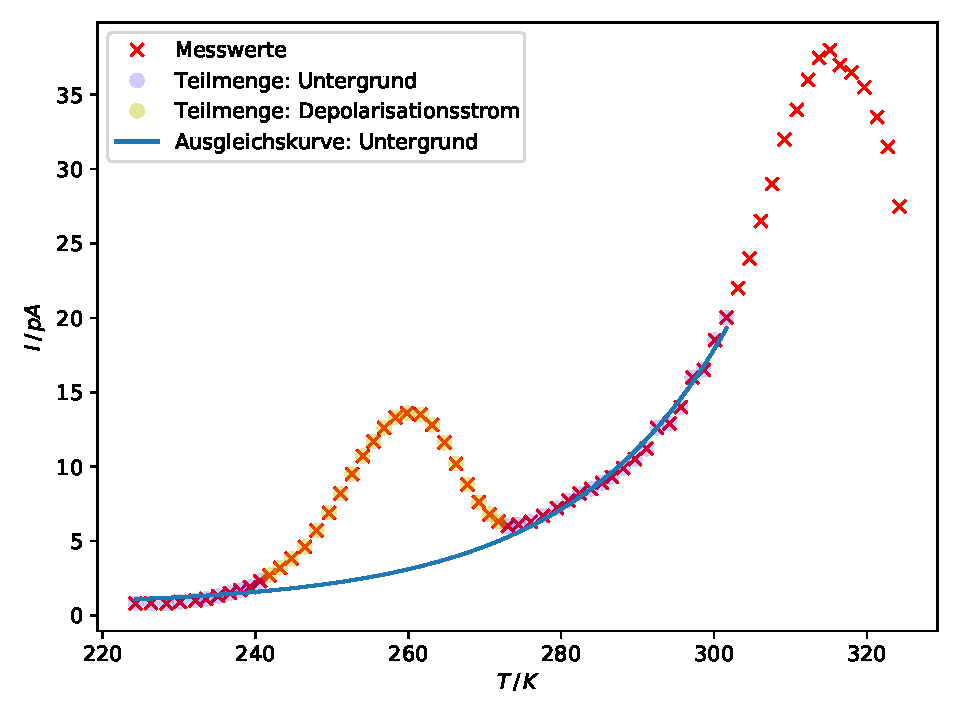
\includegraphics[width=0.7\textwidth]{content/data/T_I_kurve_15.pdf}
    \caption{Heizstrom $I$ in Abhängigkeit der Temperatur $T$ für die Heizrate $b = \SI{1.5}{\frac{\kelvin}{\minute}}$. \cite{numpy}\cite{matplotlib}\cite{scipy}}
    \label{fig:strom_temp_15}
\end{figure}

\begin{figure}
    \centering
    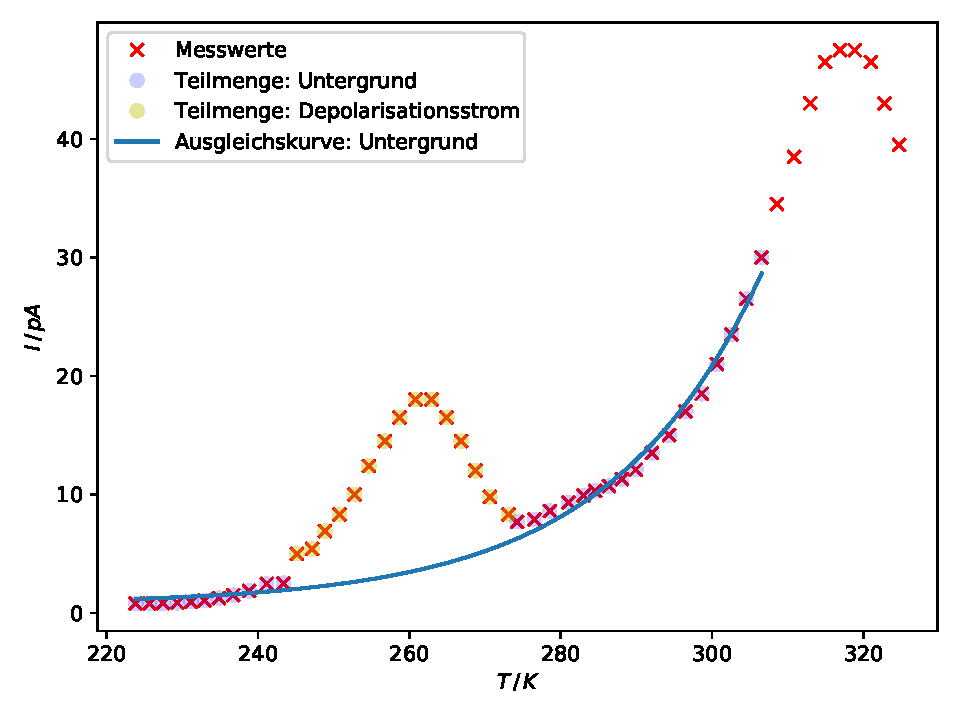
\includegraphics[width=0.7\textwidth]{content/data/T_I_kurve_20.pdf}
    \caption{Heizstrom $I$ in Abhängigkeit der Temperatur $T$ für die Heizrate $b = \SI{2.0}{\frac{\kelvin}{\minute}}$. \cite{numpy}\cite{matplotlib}\cite{scipy}}
    \label{fig:strom_temp_20}
\end{figure}
\FloatBarrier
\subsection{Berechnung der Aktivierungsenergie $W$}
Die Aktivierungsenergie $W$ für die Diffusion der Kationenleerstellen werden im folgenden Teil über die \textbf{Stromdichte} (Methode 1) und über den \textbf{Polarisationsansatz} (Methode 2) bestimmt.
Herleitung und Erklärung der Methoden können in \autoref{sec:stromdichte} bzw. \autoref{sec:polarisationsansatz} nachgelesen werden.

\subsubsection{Methode 1: Stromdichte}
Zur Berechnung der Aktivierungsenergie $W$ über die Stromdichte werden die Messwerte des Depolarisationsstroms (siehe gelb markierte Datenpunkte in \autoref{fig:strom_temp_15} bzw. \autoref{fig:strom_temp_20}) bis zum Peak verwendet.
Um den wahren Depolarisationsstrom zu erhalten muss zuerst der Untergrundstrom nach \autoref{eqn:untergrund} subtrahiert werden.
Der hier betrachtete Anfangsbereich wird durch eine exponentielle Funktion (\autoref{eq:anlauf})
\begin{equation*}
    I(T) = a \cdot \mathrm{e}^{- W / (k_B \cdot T)}
\end{equation*}
beschrieben.
Dabei stellt $a$ eine belanglose Konstante und $k_B = \SI{1.380649}{\joule \kelvin^{-1}}$\cite{constants} die Boltzmann-Konstante dar.
Aus einer Ausgleichrechnung mit dem Paket 'Scipy'\cite{scipy} für die jeweiligen Heizraten folgt die Aktivierungsenergie:
\begin{align*}
    W_{1, 1.5} &= \SI{1.26(6)e-19}{\joule} = \SI{0.79(4)}{\electronvolt} \\
    W_{1, 2.0} &= \SI{9.7(5)e-20}{\joule} = \SI{0.60(3)}{\electronvolt} \\
\end{align*}
Die verwendeten Messwerte mit Ausgleichskurve sind einem halb-logarithmischen Diagramm in \autoref{fig:approx} für die jeweiligen Heizraten aufgetragen.
\begin{figure}
    \begin{subfigure}{0.48\textwidth}
        \centering
        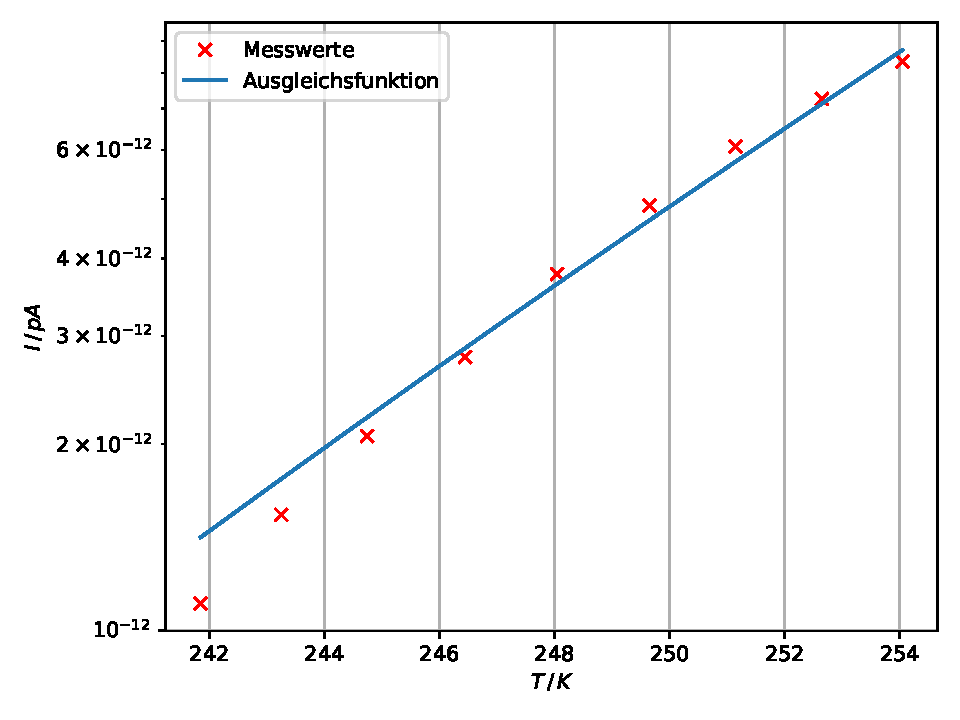
\includegraphics[height=0.8\textwidth]{content/data/W_approx_15.pdf}
        \caption{Heizrate: $b = \SI{1.5}{\kelvin \per \minute}$}
        \label{subfig:approx_15}
    \end{subfigure}
    \hfill
    \begin{subfigure}{0.48\textwidth}
        \centering
        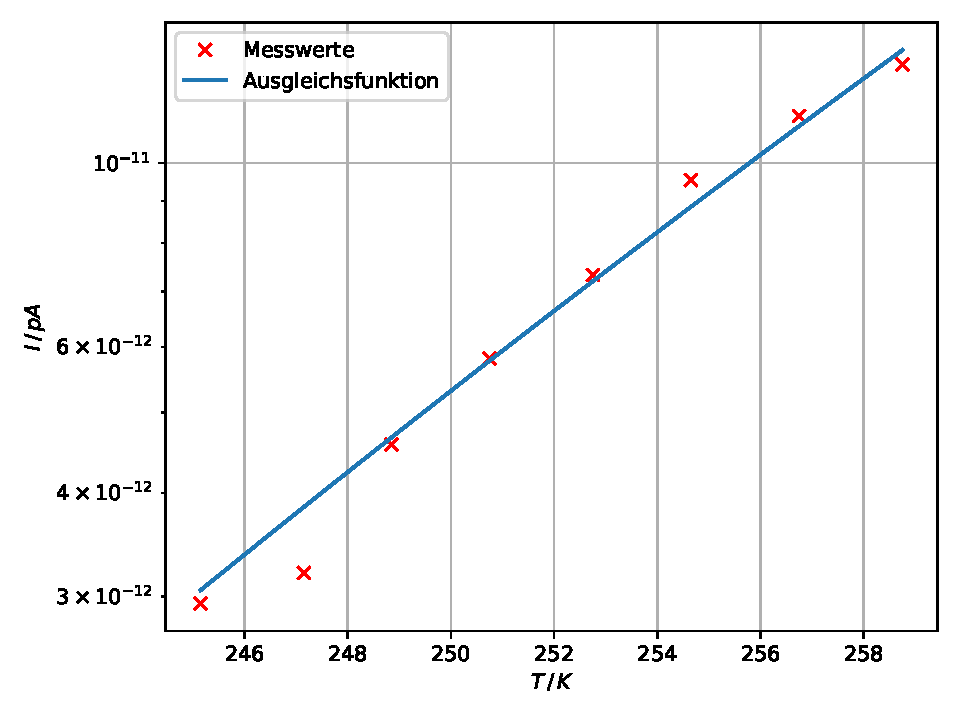
\includegraphics[height=0.8\textwidth]{content/data/W_approx_20.pdf}
        \caption{Heizrate: $b = \SI{2.0}{\kelvin \per \minute}$}
        \label{subfig:approx_20}
    \end{subfigure}
    \caption{Der Anstieg des Polarisationsstroms $I$ in Abhängigkeit der Temperatur $T$ in einem halb-logarithmischen Diagramm dargestellt.\cite{matplotlib}\cite{scipy}\cite{numpy}}
    \label{fig:approx}
\end{figure}
\FloatBarrier

\subsection{Methode 2: Polarisationsansatz}
Zur Berechnung der Aktivierungsenergie $W$ über den Polarisationsansatz werden alle Datenpunkte zum Depolarisationsstrom (siehe \autoref{fig:strom_temp_15} bzw. \autoref{fig:strom_temp_20}) verwendet.
Wie zuvor muss der Untergrundstrom von dem Depolarisationsstrom abgezogen werden.
Es folgt eine lineare Ausgleichsrechnung
\begin{equation*}
    a \cdot x + c = y
\end{equation*}
nach \autoref{eq:int} mit folgenden Definitionen:
\begin{align*}
    x &\coloneqq \frac{1}{T} \\
    y &\coloneqq \ln \frac{ \int_{T}^{\infty} I(T')\symup{d}T'}{I(T')} \\
    a &\coloneqq W/k_B \\
    c &\coloneqq -\ln (\tau_0 b)
\end{align*}
Die Integration wird nummerisch nach der Simpsonschen Formel mit der Phython-Bibliothek 'scipy'\cite{scipy} durchgeführt.
Die Parameter $a, c$ ergeben sich für die jeweiligen Heizraten zu
\begin{align*}
    a_{1.5} &= \SI{8.46(30)e+03}{\kelvin} \, ,\\
    c_{1.5} &= \SI{-30.3(12)}{} \, , \\
    \\
    a_{2.0} &= \SI{1.026(20)e+04}{\kelvin} \, , \\
    c_{2.0} &= \SI{-37.3(8)}{} \, .
\end{align*}
Die Ausgleichskurve für beide Heizraten mit den zugehörigen Messpunkten ist in \autoref{fig:int_ergebnisse} zu sehen.
Aus dem Parameter $a$ folgt umgehend die Aktivierungsenergie:
\begin{align*}
    W_{2, 1.5} &= \SI{1.17(4)e-19}{\joule} = \SI{0.729(26)}{\electronvolt} \\
    W_{2, 2.0} &= \SI{1.416(28)e-19}{\joule} = \SI{0.884(17)}{\electronvolt} \\
\end{align*}

\begin{figure}
    \begin{subfigure}{0.48\textwidth}
        \centering
        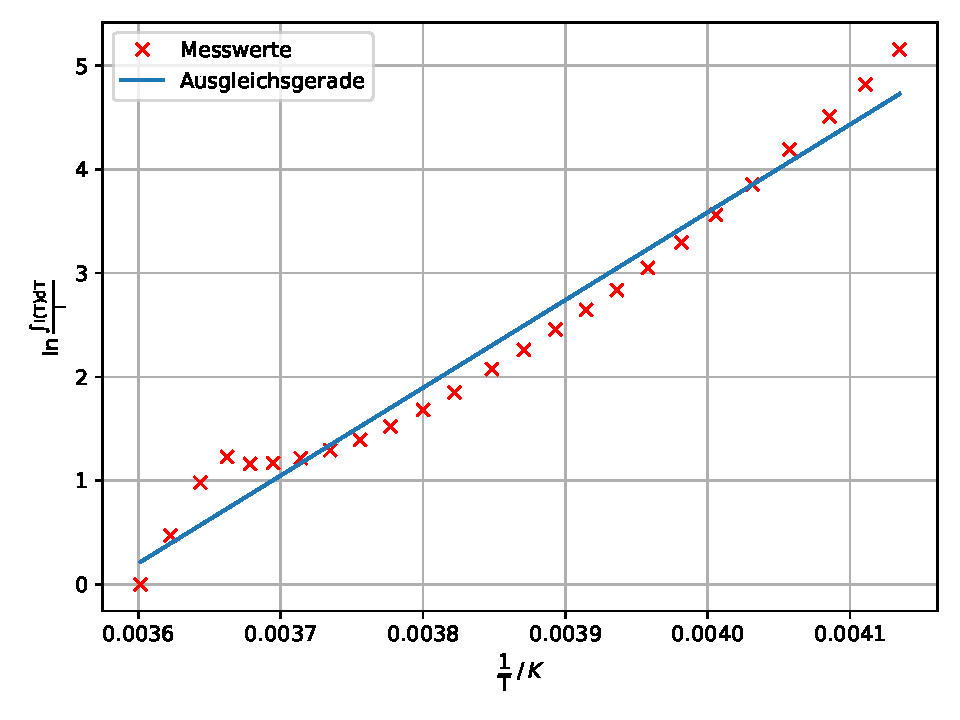
\includegraphics[height=0.8\textwidth]{content/data/integration_15.pdf}
        \caption{Heizrate: $b = \SI{1.5}{\kelvin \per \minute}$}
        \label{subfig:int_15}
    \end{subfigure}
    \hfill
    \begin{subfigure}{0.48\textwidth}
        \centering
        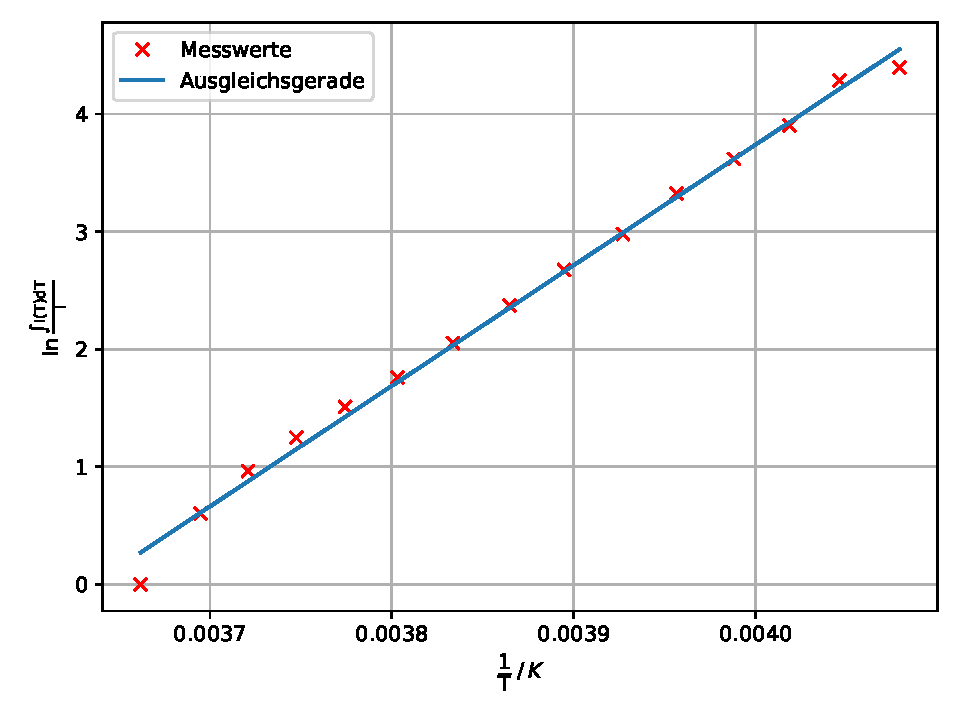
\includegraphics[height=0.8\textwidth]{content/data/integration_20.pdf}
        \caption{Heizrate: $b = \SI{2.0}{\kelvin \per \minute}$}
        \label{subfig:int_20}
    \end{subfigure}
    \caption{Ausgleichskurve zur Bestimmung der Aktivierungsenergie $W = a \cdot k_B$ mit Steigung $a$ nach Methode 2.\cite{matplotlib}\cite{scipy}\cite{numpy}}
    \label{fig:int}
\end{figure}
\FloatBarrier

\subsection{Die charakteristische Relaxationszeit \texorpdfstring{$\tau_0$}{tau0}}
Zur Bestimmung der charakteristischen Relaxationszeit wird zuerst die wahre Heizrate bestimmt.
Dazu wird eine Ausgleichsgerade durch die Zeit-Temperatur-Wertepaare gelegt, wobei die Steigung die Heizrate angibt.
Die zur Ausgleichsgerade
\begin{equation*}
    T(t) = b \cdot t + c
\end{equation*}
bestimmten Koeffizienten betragen für $b_\text{th} = \SI{1.5}{\kelvin \per \minute}$
\begin{align*}
    b_{1.5} &= \SI{1.4918(19)}{\kelvin \per \minute} \, , \\
    c_{1.5} &= \SI{225.64(7)}{\kelvin} 
\end{align*}
bzw. für $b_\text{th} = \SI{2.0}{\kelvin \per \minute}$
\begin{align}
    b_{2.0} &= \SI{1.9875(29)}{\kelvin \per \minute} \, , \\
    c_{2.0} &= \SI{223.13(9)}{\kelvin} \, .
\end{align}
Die Ergebnisse sind graphisch in \autoref{subfig:t_T_15} bzw. \autoref{subfig:t_T_20} dargestellt.
\begin{figure}
    \begin{subfigure}{0.48\textwidth}
        \centering
        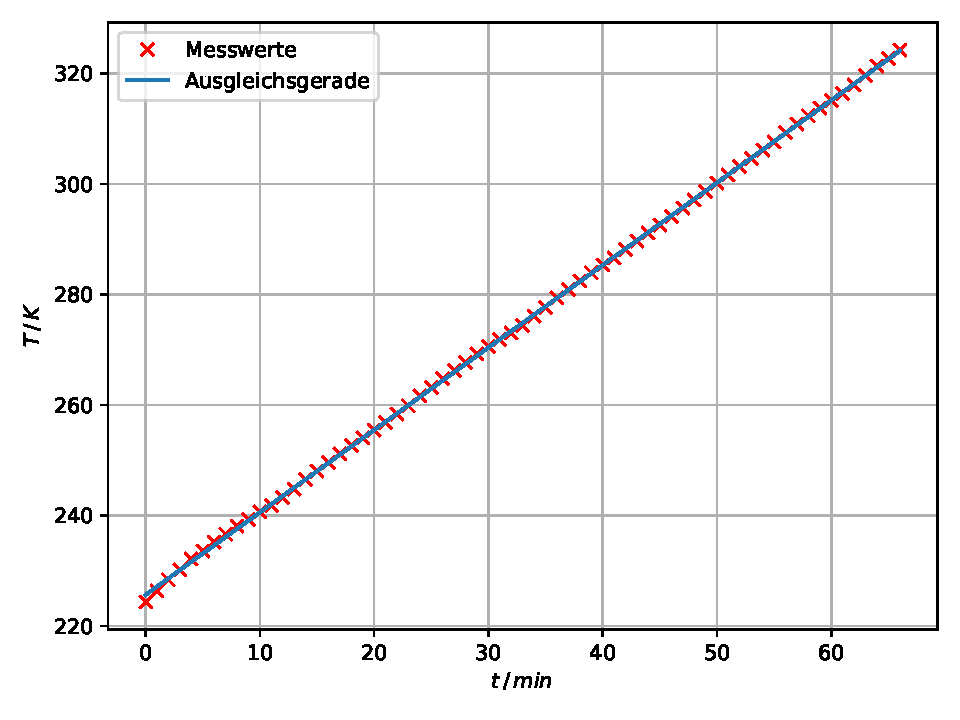
\includegraphics[height=0.8\textwidth]{content/data/char_relaxationszeit_15.pdf}
        \caption{Heizrate: $b_\text{th} = \SI{1.5}{\kelvin \per \minute}$}
        \label{subfig:t_T_15}
    \end{subfigure}
    \hfill
    \begin{subfigure}{0.48\textwidth}
        \centering
        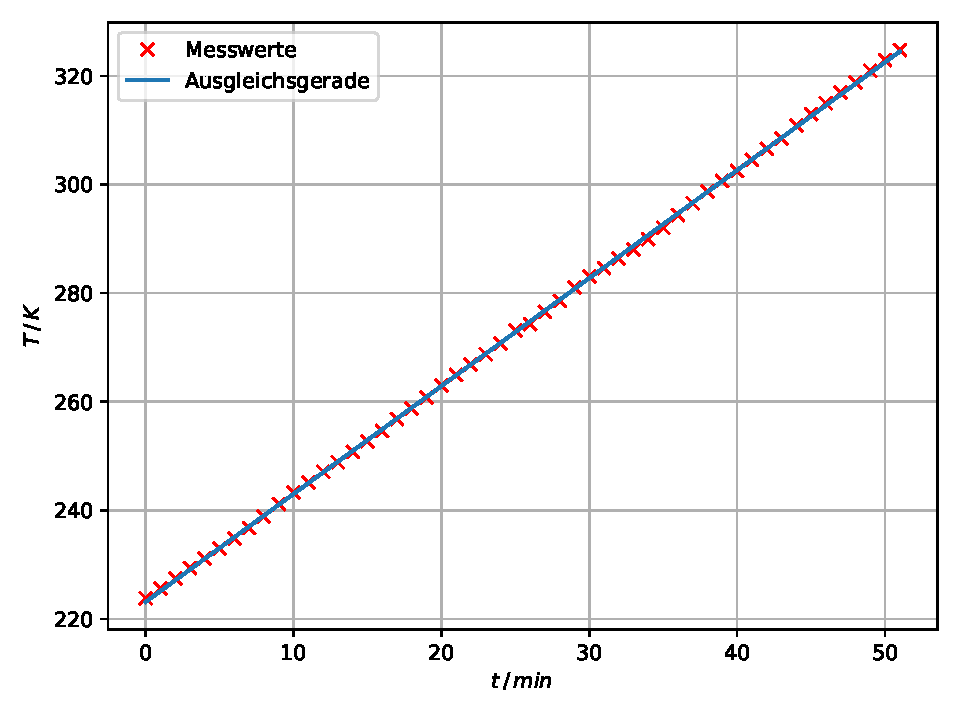
\includegraphics[height=0.8\textwidth]{content/data/char_relaxationszeit_20.pdf}
        \caption{Heizrate: $b_\text{th} = \SI{2.0}{\kelvin \per \minute}$}
        \label{subfig:t_T_20}
    \end{subfigure}
    \caption{Die Steigung der Ausgleichgerade im Temperatur-Zeit-Diagramm entspricht der Heizrate $b$.\cite{matplotlib}\cite{scipy}\cite{numpy}}
    \label{fig:int}
\end{figure}
\FloatBarrier
Nun wird die maximale Temperatur $T_\text{max}$ aus den Daten entnommen und nach \autoref{eq:t_max} die Relaxationszeit $\tau(T_\text{max})$ für die jeweiligen Heizraten und Methoden bestimmt.
Aus der Aktivierungsenergie $W$, den Wertepaaren $T_\text{max}$ und $\tau(T_\text{max})$ kann nach \autoref{eq:Relaxationszeit} die charakteristische Relaxationszeit ermittelt werden.
Die Ergebnisse sind in \autoref{tab:char_relax_15} und \autoref{tab:char_relax_20} aufgeführt.
\begin{table}
    \centering
    \caption{Die charakteristische Relaxationszeit $\tau_0$ und die zur Berechnung verwendeten Werte für den ersten Datensatz $b_\text{th} = \SI{1.5}{\kelvin \per \minute}$.}
    \label{tab:char_relax_15}
    \begin{tabular}{c | c c c c | c}
        \toprule
        & $b \,/\, \si{\frac{\kelvin}{\minute}}$ & $T_\text{max} \,/\, \si{\kelvin}$ & $W \,/\, \si{\electronvolt}$ & $\tau(T_\text{max}) \,/\, \si{\second}$ & $\tau_0 \,/\, \si{\second}$ \\
        \midrule
        Methode 1 & $\SI{1.4918(19)}{}$ & $260$ & $\SI{0.79(4)}{}$ & $\SI{298(14)}{}$ & $\SI{1.7(29)e-13}{}$ \\
        Methode 2 & $\SI{1.4918(19)}{}$ & $260$ & $\SI{0.729(26)}{}$ & $\SI{321(11)}{}$ & $\SI{2.2(26)e-12}{}$ \\
        \bottomrule
    \end{tabular}
\end{table}

\begin{table}
    \centering
    \caption{Die charakteristische Relaxationszeit $\tau_0$ und die zur Berechnung verwendeten Werte für den zweiten Datensatz $b_\text{th} = \SI{2.0}{\kelvin \per \minute}$.}
    \label{tab:char_relax_20}
    \begin{tabular}{c | c c c c | c}
        \toprule
        & $b \,/\, \si{\frac{\kelvin}{\minute}}$ & $T_\text{max} \,/\, \si{\kelvin}$ & $W \,/\, \si{\electronvolt}$ & $\tau(T_\text{max}) \,/\, \si{\second}$ & $\tau_0 \,/\, \si{\second}$ \\
        \midrule
        Methode 1 & $\SI{1.9875(29)}{}$ & $262$ & $\SI{0.60(3)}{}$ & $\SI{298(16)}{}$ & $\SI{0.9(13)e-09}{}$ \\
        Methode 2 & $\SI{1.9875(29)}{}$ & $262$ & $\SI{0.884(17)}{}$ & $\SI{203(4)}{}$ & $\SI{2.3(19)e-15}{}$ \\
        \bottomrule
    \end{tabular}
\end{table}
\FloatBarrier

\newpage
\subsection{Verlauf der Relaxationszeit \texorpdfstring{$\tau (T)$}{tau von T}}
Zuletzt wird der Verlauf der Relaxationszeit $\tau(T)$ in Abhängigkeit der Temperatur $T$ für beide Methoden und Heizraten in \autoref{fig:tau_von_T} dargestellt.
\begin{figure*}
    \centering
    \begin{subfigure}[b]{0.475\textwidth}
        \centering
        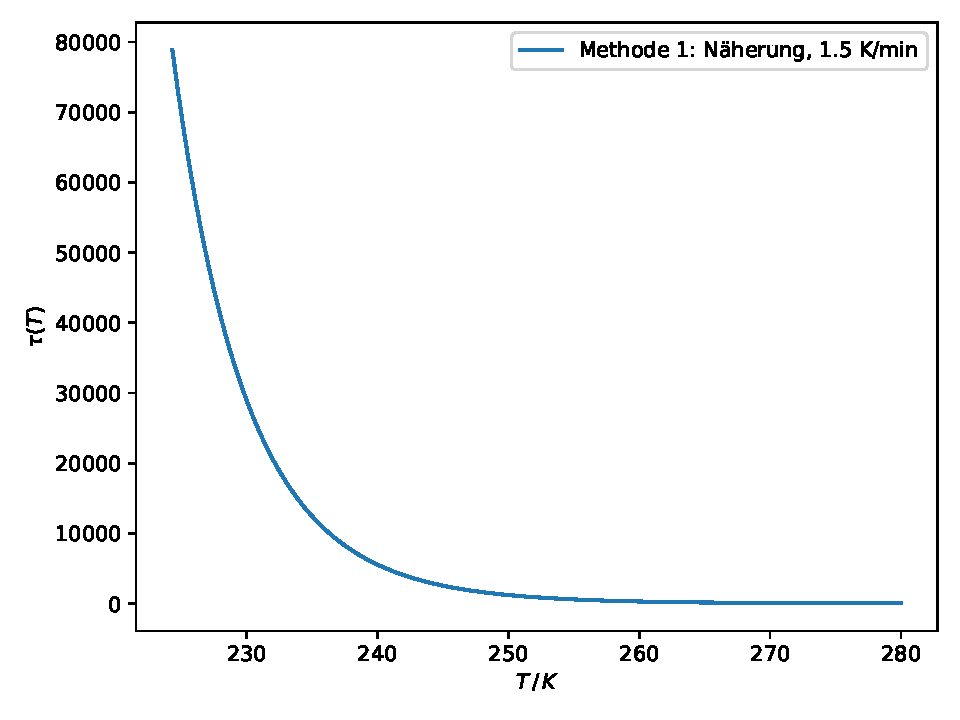
\includegraphics[width=\textwidth]{content/data/relaxationszeit_approx_15.pdf}
        \caption[]%
        {{\small Methode 1, $b = \SI{1.5}{\kelvin \per \minute}$}}    
        \label{fig:mean and std of net14}
    \end{subfigure}
    \hfill
    \begin{subfigure}[b]{0.475\textwidth}  
        \centering 
        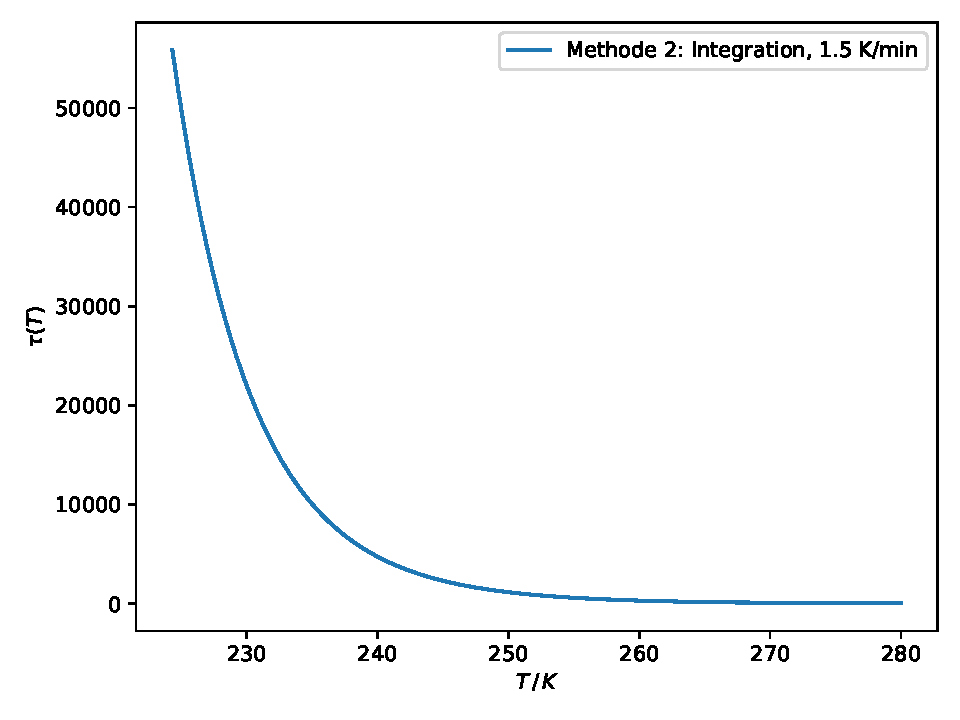
\includegraphics[width=\textwidth]{content/data/relaxationszeit_int_15.pdf}
        \caption[]%
        {{\small Methode 2, $b = \SI{1.5}{\kelvin \per \minute}$}}    
        \label{fig:mean and std of net24}
    \end{subfigure}
    \vskip\baselineskip
    \begin{subfigure}[b]{0.475\textwidth}   
        \centering 
        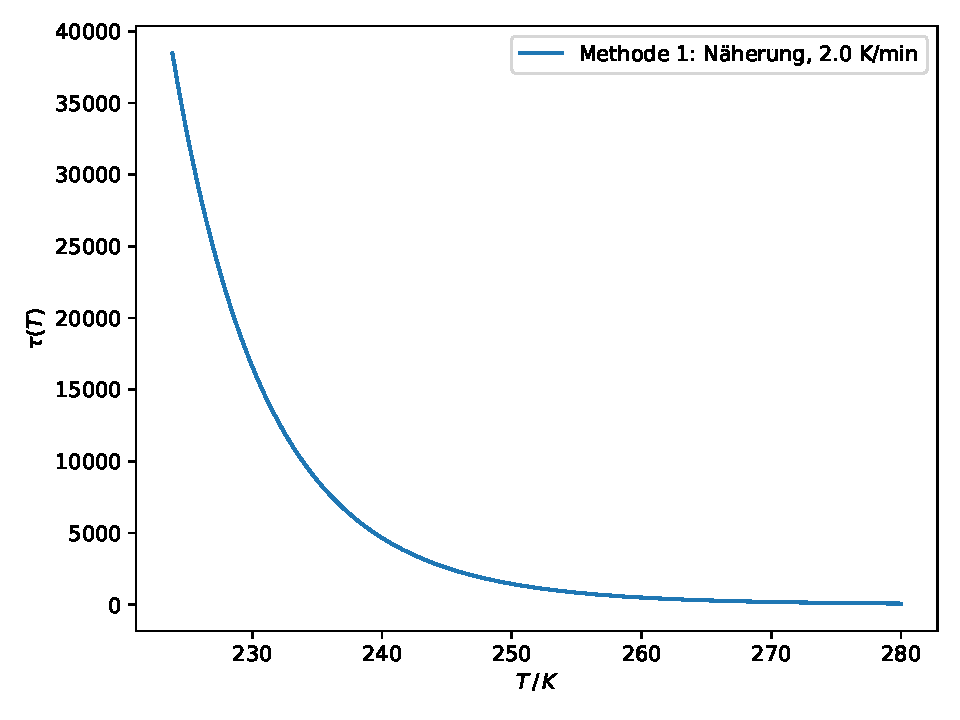
\includegraphics[width=\textwidth]{content/data/relaxationszeit_approx_20.pdf}
        \caption[]%
        {{\small Methode 1, $b = \SI{2.0}{\kelvin \per \minute}$}}    
        \label{fig:mean and std of net34}
    \end{subfigure}
    \hfill
    \begin{subfigure}[b]{0.475\textwidth}   
        \centering 
        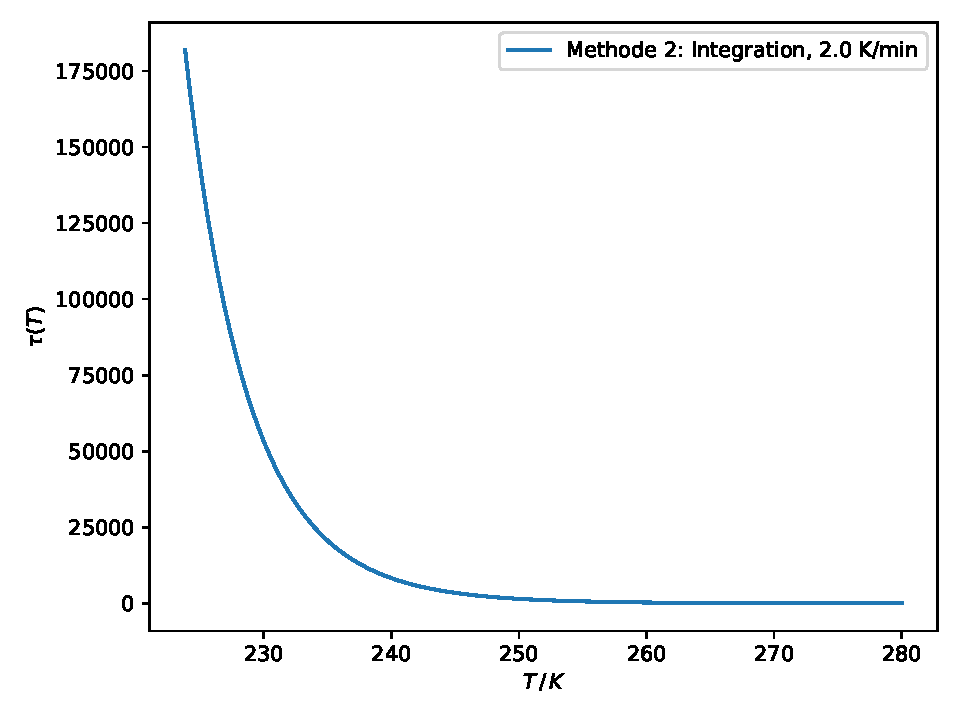
\includegraphics[width=\textwidth]{content/data/relaxationszeit_int_20.pdf}
        \caption[]%
        {{\small Methode 2, $b = \SI{2.0}{\kelvin \per \minute}$}}    
        \label{fig:mean and std of net44}
    \end{subfigure}
    \caption[ The average and standard deviation of critical parameters ]
    {\small Die Relaxationszeit $\tau (T)$ für beide Methoden und Heizraten $b$ aufgetragen.\cite{numpy}\cite{matplotlib}} 
    \label{fig:tau_von_T}
\end{figure*}